%
% My Resume Template
%

\documentclass[10pt,a4paper,landscape]{article}
\usepackage[utf8]{inputenc}

% Graphics packages
\usepackage{graphicx}
\usepackage{color}

% Use the whole page and save tree.
\usepackage[margin=2cm]{geometry}

% Better typesetting calculations
\usepackage{microtype}
\usepackage[T1]{fontenc}

% Modify fonts.
\renewcommand{\rmdefault}{cmss}
\usepackage[bitstream-charter]{mathdesign}
\usepackage[T1]{fontenc}

% Spaces instead of indentation for paragraphs.
\setlength{\parindent}{0pt}
\setlength{\parskip}{1mm plus 1mm minus 1mm}

% No page numbers
\pagenumbering{gobble}

% Columns
\usepackage{multicol}

% Staple mark :)
\usepackage{eso-pic}
\AddToShipoutPictureBG{
  \put(790,545){{
\includegraphics[scale=0.8]{staple.png}}}
}

\newcommand{\myurl}[1] {
  \mbox{[ #1 ]}
}

\begin{document}

\setlength{\columnsep}{4cm}

\begin{multicols}{2}

\vspace*{60mm}

\begin{center}
  \begin{minipage}{60mm}
    \centering
    Kangaroo Point Cliffs \\
    Sport Climbing Map
  \end{minipage}
\end{center}

\begin{center}
  \begin{minipage}{60mm}
    \centering
    Download a copy from \myurl{azrac.net/kangaroo-point}.
    It'll work best (and save a few trees) if you print double sided, flipping on the short edge.
  \end{minipage}
\end{center}

%\vspace*{20mm}

\begin{center}
  \begin{minipage}{60mm}
    \centering
    Suggestions and corrections can be mailed to \myurl{climbing@azrac.net}.
  \end{minipage}
\end{center}

%\vspace*{20mm}

\begin{center}
  \begin{minipage}{60mm}
    \centering
    This is a free map but if you appreciate it, it's always nice to hear some thanks!
  \end{minipage}
\end{center}

\vspace*{20mm}

\vfill
\columnbreak




{\bf\Huge Kangaroo Point Cliffs}

{\Large Sport Climbing}

\vspace{5mm}

\normalsize

The Kangaroo Point Cliffs offer great climbing right in the center of Brisbane.
This is a simple, clean and concise map of the main sport climbing routes in the area.
Convenient and easy to carry!
To find detailed information about the routes take a look at the website `The Crag'.
\myurl{thecrag.com/climbing/australia/kangaroo-point}

\begin{center}
  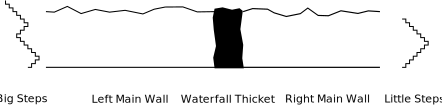
\includegraphics[scale=0.7]{map.png}
\end{center}

The cliffs are divided into two sections, separated by a thicket of trees with an (occasional) waterfall.
At either end of the wall there are steps up to the top.
Here you can find plenty of rings and bollards to abseil from or use to build a top-rope anchor.

\begin{center}
  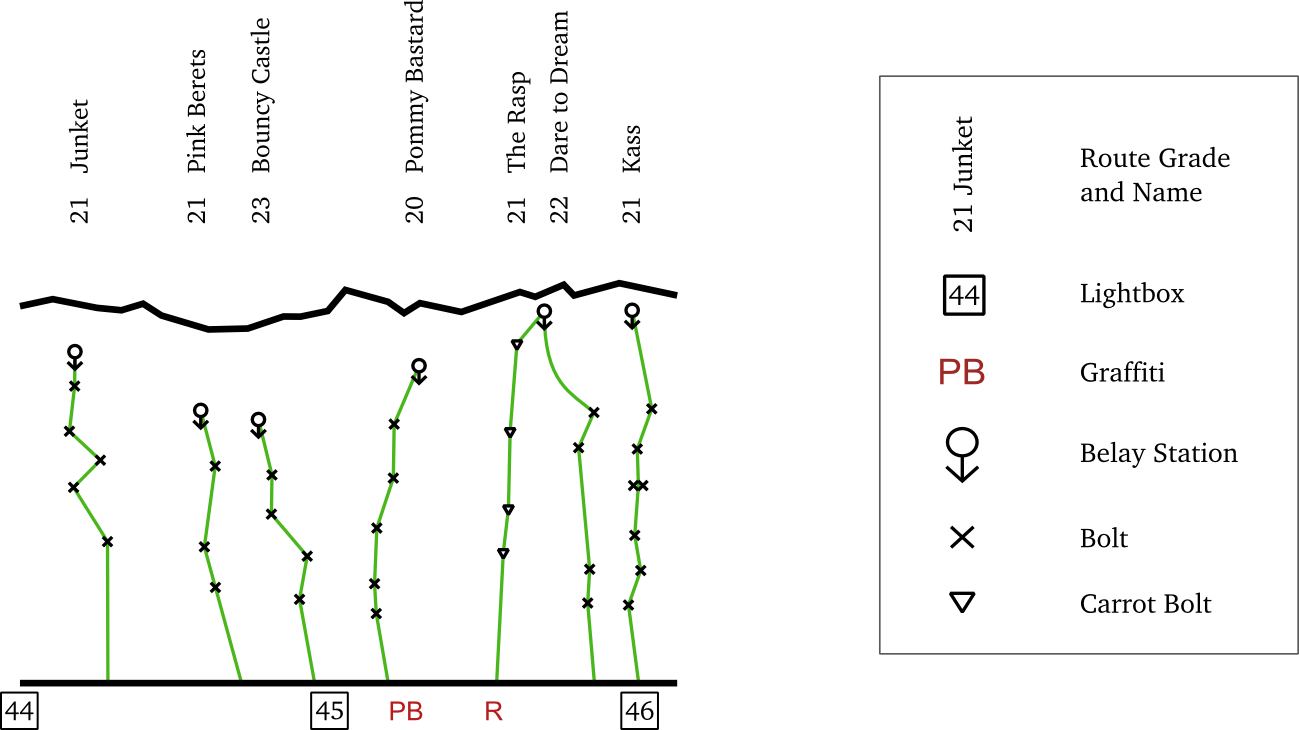
\includegraphics[scale=0.7]{legend.png}
\end{center}

Keep an eye out when throwing ropes down and check there isn't someone below.
Try to use your own gear to lower from whenever possible, it keeps everything spick and spam.
Have fun!



\end{multicols}


\end{document}
